\documentclass{beamer}
\usepackage[utf8]{inputenc}

\usetheme{Madrid}
\usecolortheme{default}
\usepackage{amsmath,amssymb,amsfonts,amsthm}
\usepackage{txfonts}
\usepackage{tkz-euclide}
\usepackage{listings}
\usepackage{adjustbox}
\usepackage{array}
\usepackage{tabularx}
\usepackage{gvv}
\usepackage{lmodern}
\usepackage{circuitikz}
\usepackage{tikz}
\usepackage{graphicx}

\setbeamertemplate{page number in head/foot}[totalframenumber]

\usepackage{tcolorbox}
\tcbuselibrary{minted,breakable,xparse,skins}



\definecolor{bg}{gray}{0.95}
\DeclareTCBListing{mintedbox}{O{}m!O{}}{%
  breakable=true,
  listing engine=minted,
  listing only,
  minted language=#2,
  minted style=default,
  minted options={%
    linenos,
    gobble=0,
    breaklines=true,
    breakafter=,,
    fontsize=\small,
    numbersep=8pt,
    #1},
  boxsep=0pt,
  left skip=0pt,
  right skip=0pt,
  left=25pt,
  right=0pt,
  top=3pt,
  bottom=3pt,
  arc=5pt,
  leftrule=0pt,
  rightrule=0pt,
  bottomrule=2pt,
  toprule=2pt,
  colback=bg,
  colframe=orange!70,
  enhanced,
  overlay={%
    \begin{tcbclipinterior}
    \fill[orange!20!white] (frame.south west) rectangle ([xshift=20pt]frame.north west);
    \end{tcbclipinterior}},
  #3,
}
\lstset{
    language=C,
    basicstyle=\ttfamily\small,
    keywordstyle=\color{blue},
    stringstyle=\color{orange},
    commentstyle=\color{green!60!black},
    numbers=left,
    numberstyle=\tiny\color{gray},
    breaklines=true,
    showstringspaces=false,
}

\title{1.4.26}
\subtitle{Vector Section Formula}
\author{EE25BTECH11010 - Arsh Dhoke}
\date{}

\begin{document}

\begin{frame}
\titlepage
\end{frame}

\begin{frame}{Question}
The position vector of the point which divides the join of points 
$2\vec{a} - 3\vec{b}$ and $\vec{a} + \vec{b}$
in the ratio $3:1$ is \underline{\hspace{2cm}}.
\end{frame}

\begin{frame}{Theoretical Solution}

\begin{align}
    \vec{P} &= 2\vec{a}-3\vec{b},  \label{eq:1} \\ 
    \vec{Q} &= \vec{a}+\vec{b}. \label{eq:2}
\end{align}

Now, the matrix form for $\vec{Q}$ and $\vec{P}$ is:
\begin{align}
\myvec{\vec{Q} & \vec{P}}
= \myvec{\vec{a} & \vec{b}}
\myvec{1 & 2 \\ 1 & -3}. \label{eq:3}
\end{align}
\end{frame}

\begin{frame}{Equation}
Using section formula, the point $\vec{R}$ dividing $\vec{Q} - \vec{P}$ in ratio $3:1$ is:

\begin{align}
\vec{R} &= \frac{3\vec{Q} + 1\vec{P}}{3+1} \label{eq:4} \\
\vec{R} &= \frac{1}{4} \cdot \myvec{\vec{Q} & \vec{P}} \myvec{3 \\ 1}\label{eq:5} \\
\vec{R} &= \frac{1}{4} \cdot \myvec{\vec{a} & \vec{b}}\myvec{1 & 2 \\ 1 & -3} \myvec{3 \\ 1} \label{eq:6} 
\end{align}

\end{frame}

\begin{frame}{Calculation Steps}
\begin{align}
\vec{R} &= \frac{1}{4} \cdot \myvec{\vec{a} & \vec{b}} \myvec{5 \\ 0} \label{eq:7} \\
\vec{R} &= \frac{1}{4} \cdot \myvec{5\vec{a}} \label{eq:8} 
\end{align}
\end{frame}

\begin{frame}{Plot}
\centering
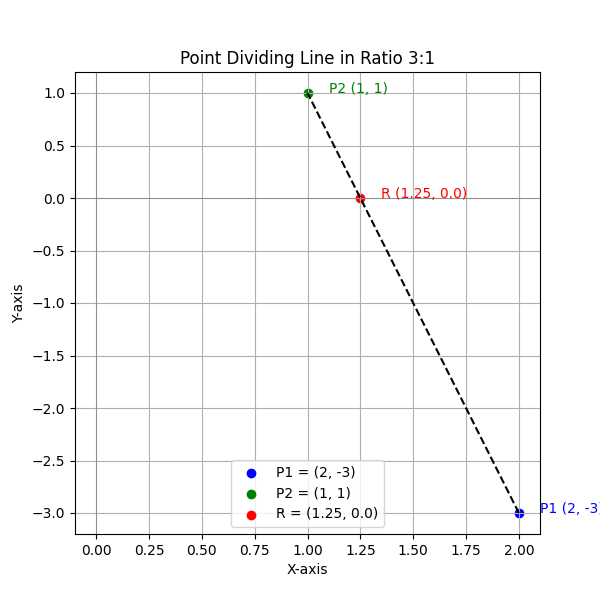
\includegraphics[height=0.7\textheight, keepaspectratio]{figs/q1.png}
\end{frame}

\begin{frame}[fragile]
    \frametitle{C Code - Section formula}

    \begin{lstlisting}
#include <stdio.h>

void sectionFormula(int m, int n, float a, float b, float *x) {
    *x = (m * b + n * a) / (float)(m + n);
}

    \end{lstlisting}
\end{frame}

\begin{frame}[fragile]
    \frametitle{Python Code}

    \begin{lstlisting}
import numpy as np
import matplotlib.pyplot as plt

# Define values for a and b
a = 1  # Example value
b = 0  # Example value

# Define points as NumPy arrays
P = np.array([2*a, -3*b])  # Point P
Q = np.array([a, b])       # Point Q

# Ratio m:n
m = 3
n = 1

# Section formula for internal division
R = (m * Q + n * P) / (m + n)

# Print the result
print("Position vector of the point R:", R)

    \end{lstlisting}
\end{frame}

\begin{frame}[fragile]
    \frametitle{Python Code}

    \begin{lstlisting}

# Plotting
plt.figure(figsize=(6, 6))
plt.axhline(0, color='black', linewidth=0.8)
plt.axvline(0, color='black', linewidth=0.8)

# Plot P, Q, and R
plt.scatter(*P, color='blue', label='P (2a, -3b)')
plt.scatter(*Q, color='green', label='Q (a, b)')
plt.scatter(*R, color='red', label=f'R (ratio {m}:{n})')

# Draw line between P and Q
plt.plot([P[0], Q[0]], [P[1], Q[1]], color='gray', linestyle='--')

# Annotate points
plt.text(P[0]+0.2, P[1]+0.2, 'P')
plt.text(Q[0]+0.2, Q[1]+0.2, 'Q')
plt.text(R[0]+0.2, R[1]+0.2, 'R')

\end{lstlisting}
\end{frame}


\begin{frame}[fragile]
    \frametitle{Python Code}

    \begin{lstlisting}

plt.xlabel('X-axis')
plt.ylabel('Y-axis')
plt.title('Section Formula Visualization')
plt.legend()
plt.grid(True)
plt.savefig("/home/arsh-dhoke/ee1030-2025/ee25btech11010/matgeo/1.4.26/figs/q1.png")
plt.show()

    \end{lstlisting}
\end{frame}

\begin{frame}[fragile]
    \frametitle{Python+ C Code}

    \begin{lstlisting}

import ctypes
import numpy as np
import matplotlib.pyplot as plt

# Load the shared library
lib = ctypes.CDLL("./libsection_int.so")

# Define argument and return types
lib.sectionFormula.argtypes = [
    ctypes.c_int, ctypes.c_int,
    ctypes.POINTER(ctypes.c_double), ctypes.POINTER(ctypes.c_double),
    ctypes.POINTER(ctypes.c_double)
]
lib.sectionFormula.restype = None

# Values for a and b
a = 1
b = 0


    \end{lstlisting}
\end{frame}

\begin{frame}[fragile]
    \frametitle{Python+ C Code}

    \begin{lstlisting}
    
# Points P and Q
P = (ctypes.c_double * 2)(2 * a, -3 * b)
Q = (ctypes.c_double * 2)(a, b)
R = (ctypes.c_double * 2)(0.0, 0.0)

# Ratio m:n
m, n = 3, 1

# Call the C function
lib.sectionFormula(m, n, P, Q, R)

# Convert to NumPy arrays for plotting
P_np = np.array([P[0], P[1]])
Q_np = np.array([Q[0], Q[1]])
R_np = np.array([R[0], R[1]])

print("Position vector of the point R (from C):", R_np)

  \end{lstlisting}
\end{frame}

\begin{frame}[fragile]
    \frametitle{Python+ C Code}

    \begin{lstlisting}

# Plotting
plt.figure(figsize=(6, 6))
plt.axhline(0, color='black', linewidth=0.8)
plt.axvline(0, color='black', linewidth=0.8)

# Plot P, Q, and R
plt.scatter(*P_np, color='blue', label='P (2a, -3b)')
plt.scatter(*Q_np, color='green', label='Q (a, b)')
plt.scatter(*R_np, color='red', label=f'R (ratio {m}:{n})')

# Draw line between P and Q
plt.plot([P_np[0], Q_np[0]], [P_np[1], Q_np[1]], color='gray', linestyle='--')

# Annotate points
plt.text(P_np[0]+0.2, P_np[1]+0.2, 'P')
plt.text(Q_np[0]+0.2, Q_np[1]+0.2, 'Q')
plt.text(R_np[0]+0.2, R_np[1]+0.2, 'R')

\end{lstlisting}
\end{frame}

\begin{frame}[fragile]
    \frametitle{Python+ C Code}

    \begin{lstlisting}

plt.xlabel('X-axis')
plt.ylabel('Y-axis')
plt.title('Section Formula Visualization (Using C & Python)')
plt.legend()
plt.grid(True)
plt.axis('equal')

# Save the plot
plt.savefig("/home/arsh-dhoke/ee1030-2025/ee25btech11010/matgeo/1.4.26/figs/q1.png")

# Show plot
plt.show()


      \end{lstlisting}
\end{frame}

\end{document}
